\clearpage
\state{(Jackson 12.15)}{
	Consider the Proca equation for a localized steady-state distribution of current that has only a static magnetic moment.  This model can be used to study the observable effects of a finite photon mass on the earth's magnetic field.  Note that if the magnetization is $\vcM(\vx)$ the current density can be written as $\vJ = c \,(\grad \cross \vcM)$.
}

%
%	Jackson 12.15(a)
%

\prob{}{
	Show that if $\vcM = \vm \,f(\vx)$, where $\vm$ is a fixed vector and $f(\vx)$ is a localized scalar function, the vector potential is
	\eq{
		\vA(\vx) = -\vm \cross \grad \int f(\vx') \frac{e^{-\mu \abs{\vx - \vx'}}}{\abs{\vx - \vx'}} \ddcxp.
	}
	\vfix
}

\sol{
	The Proca equations of motion in the static limit are given by the equation immediately following Jackson~(12.93),
	\eq{
		\lap \Asa - \mu^2 \Asa = -\frac{4\pi}{c} \Jsa,
	}
	which implies
	\eqn{thing3}{	
		\lap \vA - \mu^2 \vA = -\frac{4\pi}{c} \vJ.
	}
	We will proceed by finding the Green's function for this equation, which satisfies
	\eqn{green}{
		(\lap - \mu^2) \,G(\vx) = \del^3(\vx).
	}
	We can Fourier transform $G(\vx)$ so long as $\vA$ and its derivatives vanish at infinity~\cite{Poisson}.  The Fourier transform expression and its inverse in one dimension are, according to Jackson~(2.45--46),
	\al{
		A(k) &= \frac{1}{\sqrt{2\pi}} \intnii e^{-i k x} \,f(x) \ddx, &
		f(x) &= \frac{1}{\sqrt{2\pi}} \intnii A(k) \,e^{i k x} \ddk.
	}
	Generalizing to three dimensions, the Green's function transforms as~\cite{Poisson}
	\eq{
		G(\vk) = \frac{1}{(2\pi)^{3/2}} \int G(\vx) \,e^{i \vk \vdot \vx} \ddcx.
	}
	Transforming both sides of Eq.~\refeq{green} in the same way, we have~\cite{Poisson}
	\al{
		\frac{1}{(2\pi)^{3/2}} \int (\lap - \mu^2) \,G(\vx) \,e^{i \vk \vdot \vx} \ddcx &= \frac{1}{(2\pi)^{3/2}} \int \lap \,G(\vx) \,e^{i \vk \vdot \vx} \ddcx - \frac{\mu^2}{(2\pi)^{3/2}} \int G(\vx) \,e^{i \vk \vdot \vx} \ddcx \\
		&= \frac{k^2 - \mu^2}{(2\pi)^{3/2}}  \int G(\vx) \,e^{i \vk \vdot \vx} \ddcx, \\[1.5ex]
		\frac{1}{(2\pi)^{3/2}} \int \del^3(\vx) \,e^{i \vk \vdot \vx} \ddcx &= \frac{1}{(2\pi)^{3/2}},
	}
	so
	\eq{
		(k^2 - \mu^2) \,G(\vk) = \frac{1}{(2\pi)^{3/2}}
		\qimplies
		G(\vk) = \frac{1}{(2\pi)^{3/2} (k^2 - \mu^2)}.
	}
	Then we can find $G(\vx)$ using the inverse Fourier transform~\cite{Poisson}:
	\al{
		G(\vx) &= \frac{1}{(2\pi)^{3/2}} \int G(\vk) \,e^{i \vk \vdot \vx} \ddck
		= \frac{1}{(2\pi)^3} \int \frac{e^{i \vk \vdot \vx}}{k^2 - \mu^2} \ddck
		= \frac{1}{(2\pi)^3} \int_0^{2\pi} \int_0^\pi \intoi \frac{e^{i k \absvx}}{k^2 - \mu^2} k^2 \sin\tht \ddk \dd{\tht} \dd{\phi} \\
		&= \frac{4\pi}{(2\pi)^3 \absvx} \intoi \frac{k \sin(k \absvx)}{k^2 - \mu^2} k^2 \ddk
		= \frac{e^{-\mu \absvx}}{4\pi \absvx}.
	}
	
	Then the solution to Eq.~\refeq{thing3} is
	\eq{
		\vA(\vx) = \frac{4\pi}{c} \int \vJ(\vx') \,G(\vx - \vx') \ddcxp
		= \frac{1}{c} \int \vJ(\vx') \frac{e^{-\mu \abs{\vx - \vx'}}}{\abs{\vx - \vx'}} \ddcxp.
	}
	Note that
	\eq{
		\frac{\vJ}{c} = \grad \cross [ \vm \,f(\vx) ]
		= \grad f(\vx) \cross \vm + f(\vx) \,\grad \cross \vm
		= \grad f(\vx) \cross \vm
		= -\vm \cross \grad f(\vx),
	}
	where we have used the identity $\grad \cross (\psi \vaa) = \grad \psi \cross \vaa + \psi \grad \cross \vaa$.  Making this substitution,
	\eqn{thing3.2}{
		\vA(\vx) = -\int \vm \cross \grad' f(\vx') \,\frac{e^{-\mu \abs{\vx - \vx'}}}{\abs{\vx - \vx'}} \ddcxp
		= -\vm \cross \int \grad' f(\vx') \,\frac{e^{-\mu \abs{\vx - \vx'}}}{\abs{\vx - \vx'}} \ddcxp.
	}
	Integrating by parts,
	\eq{
		\int \grad' f(\vx') \,\frac{e^{-\mu \abs{\vx - \vx'}}}{\abs{\vx - \vx'}} \ddcxp = \brac{ f(\vx') \grad' \frac{e^{-\mu \abs{\vx - \vx'}}}{\abs{\vx - \vx'}} }_{-\infty}^\infty - \int f(\vx') \,\grad' \frac{e^{-\mu \abs{\vx - \vx'}}}{\abs{\vx - \vx'}} \ddcxp
		= -\int f(\vx') \,\grad' \frac{e^{-\mu \abs{\vx - \vx'}}}{\abs{\vx - \vx'}} \ddcxp,
	}
	since $f(\vx)$ is a localized scalar function and therefore vanishes at infinity.  Since the Green's function depends only on $\abs{\vx - \vx'}$, we can replace $\grad'$ by $-\grad$:
	\eq{
		-\int f(\vx') \,\grad' \frac{e^{-\mu \abs{\vx - \vx'}}}{\abs{\vx - \vx'}} \ddcxp
		= \int f(\vx') \,\grad \frac{e^{-\mu \abs{\vx - \vx'}}}{\abs{\vx - \vx'}} \ddcxp
		= \grad \int f(\vx') \frac{e^{-\mu \abs{\vx - \vx'}}}{\abs{\vx - \vx'}} \ddcxp.
	}
	Making this substitution in Eq.~\refeq{thing3.2},
	\eqn{ans3a}{
		\ans{ \vA(\vx) = -\vm \cross \grad \int f(\vx') \frac{e^{-\mu \abs{\vx - \vx'}}}{\abs{\vx - \vx'}} \ddcxp, }
	}
	as desired. \qed
}

%
%	Jackson 12.15(b)
%

\prob{}{
	If the magnetic dipole is a point dipole at the origin [$f(\vx) = \del(\vx)$], show that the magnetic field away from the origin is
	\eq{
		\vB(\vx) = [ 3 \,\rh (\rh \vdot \vm) - \vm ] \paren{ 1 + \mu r + \frac{\mu^2 r^2}{3} }\frac{e^{-\mu r}}{r^3} - \frac{2}{3} \mu^2 \vm \frac{e^{-\mu r}}{r}.
	}
	\vfix
}

\sol{
	Setting $f(\vx) = \del(\vx)$ in Eq.~\refeq{ans3a},
	\eq{
		\vA(\vx) = -\vm \cross \grad \int \del(\vx') \frac{e^{-\mu \abs{\vx - \vx'}}}{\abs{\vx - \vx'}} \ddcxp
		= -\vm \cross \grad \frac{e^{-\mu \absvx}}{\absvx}.
	}
	Note that
	\eq{
		\grad \frac{e^{-\mu \absvx}}{\absvx} = \paren{ -\frac{e^{-\mu \absvx}}{\absvx^2} - \frac{\mu e^{-\mu \absvx}}{\absvx} } \vx
		= -(1 + \mu \absvx) \frac{e^{-\mu \absvx}}{\absvx^2} \xh
		= -(1 + \mu \absvx) \frac{e^{-\mu \absvx}}{\absvx^3} \vx,
	}
	so
	\eq{
		\vA(\vx) = (\vm \cross \vx) (1 + \mu \absvx) \frac{e^{-\mu \absvx}}{\absvx^2}.
	}
	
	The magnetic field is given by $\vB = \grad \cross \vA$:
	\eq{
		\vB(\vx) = \grad \cross \brac{ (\vm \cross \vx) (1 + \mu \absvx) \frac{e^{-\mu \absvx}}{\absvx^3} }
		= \grad \brac{ (1 + \mu \absvx) \frac{e^{-\mu \absvx}}{\absvx^3}} \cross (\vm \cross \vx) + (1 + \mu \absvx) \frac{e^{-\mu \absvx}}{\absvx^3} \grad \cross (\vm \cross \vx).
	}
	For the first term,
	\eq{
		\grad \brac{ (1 + \mu \absvx) \frac{e^{-\mu \absvx}}{\absvx^3}}
		= \brac{ -\mu \frac{e^{-\mu \absvx}}{\absvx^3} + (1 + \mu \absvx) \paren{ -\frac{\mu e^{- \mu \absvx}}{\absvx^3} - \frac{3 e^{-\mu \absvx}}{\absvx^4} } } \xh \\
		= -(3 + 3\mu \absvx + \mu^2 \absvx^2) \frac{e^{-\mu \absvx}}{\absvx^4} \,\xh.
	}
	Then, using the identity $\grad \cross (\vaa \cross \vbb) = \vaa (\grad \vdot \vbb) - \vbb (\grad \vdot \vaa) + (\vbb \vdot \grad) \vaa - (\vaa \vdot \grad) \vbb$,
	\eq{
		\grad \cross (\vm \cross \vx) = \vm (\grad \vdot \vx) - \vx (\grad \vdot \vm) + (\vx \vdot \grad) \vm - (\vm \vdot \grad) \vx
		= \vm (\grad \vdot \vx) - (\vm \vdot \grad) \vx.
	}
	Making these substitutions,
	\al{
		\vB(\vx) &= -(3 + 3\mu \absvx + \mu^2 \absvx^2) \frac{e ^{-\mu \absvx}}{\absvx^3} \,\xh \cross (\vm \cross \xh) + (1 + \mu \absvx) \frac{e^{-\mu \absvx}}{\absvx^3} [ \vm (\grad \vdot \xh) - (\vm \vdot \grad) \xh ] \\
		&= -(3 + 3\mu \absvx + \mu^2 \absvx^2) \frac{e^{-\mu \absvx}}{\absvx^3} [ (\xh \vdot \xh) \vm - (\xh \vdot \vm) \xh ] + 2 (1 + \mu \absvx) \frac{e^{-\mu \absvx}}{\absvx^2} \vm \\
		&= -3 \paren{ 1 + \mu \absvx + \frac{\mu^2 \absvx^2}{3} } \frac{e^{-\mu \absvx}}{\absvx^3} [ \vm - (\xh \vdot \vm) \xh ] + 2 (1 + \mu \absvx) \frac{e^{-\mu \absvx}}{\absvx^2} \vm \\
		&= [ 3 \,\xh (\xh \vdot \vm) - \vm ] \paren{ 1 + \mu \absvx + \frac{\mu^2 \absvx^2}{3} }\frac{e^{-\mu \absvx}}{\absvx^3} - \frac{2}{3} \mu^2 \vm \frac{e^{-\mu \absvx}}{\absvx}.
	}
	Letting $\xh \to \rh$ and $\absvx \to r$, we have
	\eqn{ans3b}{
		\ans{ \vB(\vx) = [ 3 \,\rh (\rh \vdot \vm) - \vm ] \paren{ 1 + \mu r + \frac{\mu^2 r^2}{3} } \frac{e^{-\mu r}}{r^3} - \frac{2}{3} \mu^2 \vm \frac{e^{-\mu r}}{r} }
	}
	as we sought to show. \qed
}

%
%	Jackson 12.15(c)
%

\prob{}{
	The result of Prob.~{3(b)} shows that at fixed $r = R$ (on the surface of the earth), the earth's magnetic field will appear as a dipole angular distribution, plus an added constant magnetic field (an apparently external field) antiparallel to $\vm$.  Satellite and surface observations lead to the conclusion that the ``external'' field is less than $\num{4e-3}$ times the dipole field at the magnetic equator.  Estimate a lower limit on $\mu^{-1}$ in earth radii and an upper limit on the photon mass in grams from this datum.
}

\sol{
	The earth's magnetic field is parallel to its surface at the magnetic equator~\cite{Magnetic}.  Figure~\ref{mag} shows the field of a magnetic dipole $\vm$ that points in the $z$ direction~\cite[pp.~245--246]{Griffiths}.  Thus, at the magnetic equator, $\vm$ is also parallel to the field, and so the spherical unit vector $\rh$ is perpendicular to $\vm$.  So Eq.~\refeq{ans3b} becomes
	\eq{
		\vB(\vx) = -\vm \paren{ 1 + \mu R + \frac{\mu^2 R^2}{3} }\frac{e^{-\mu R}}{R^3} - \frac{2}{3} \mu^2 \vm \frac{e^{-\mu R}}{R}
		\equiv \vBdip + \vBext,
	}
	where we have defined $\vBdip$ as the dipole field and $\vBext$ as the ``external' field.  The identification is made by comparing with Jackson~(5.56), which gives the magnetic field due to a dipole (in SI units):
	\eq{
		\vB(\vx) = \frac{\muo}{4\pi} \frac{3 \nh (\nh \vdot \vm)}{\absvx^3}.
	}
	As stated in the problem, $\abs{\vBext} < (\num{4e-3}) \abs{\vBdip}$.  This gives us
	\eq{
		\frac{2}{3} \mu^2 \frac{e^{-\mu R}}{R} < (\num{4e-3}) \paren{ 1 + \mu R + \frac{\mu^2 R^2}{3} } \frac{e^{-\mu R}}{R^3}
		\qimplies
		\frac{2}{3} \mu^2 R^2 < (\num{4e-3}) \paren{ 1 + \mu R + \frac{\mu^2 R^2}{3} }.
	}
	Solving the second expression with Mathematica gives the positive solution $\mu = 0.0806 / R$.  Thus, the lower limit on $\mu^{-1}$ is \ans{$\mu^{-1} > 12 R$.}
	
	\begin{figure} \centering
		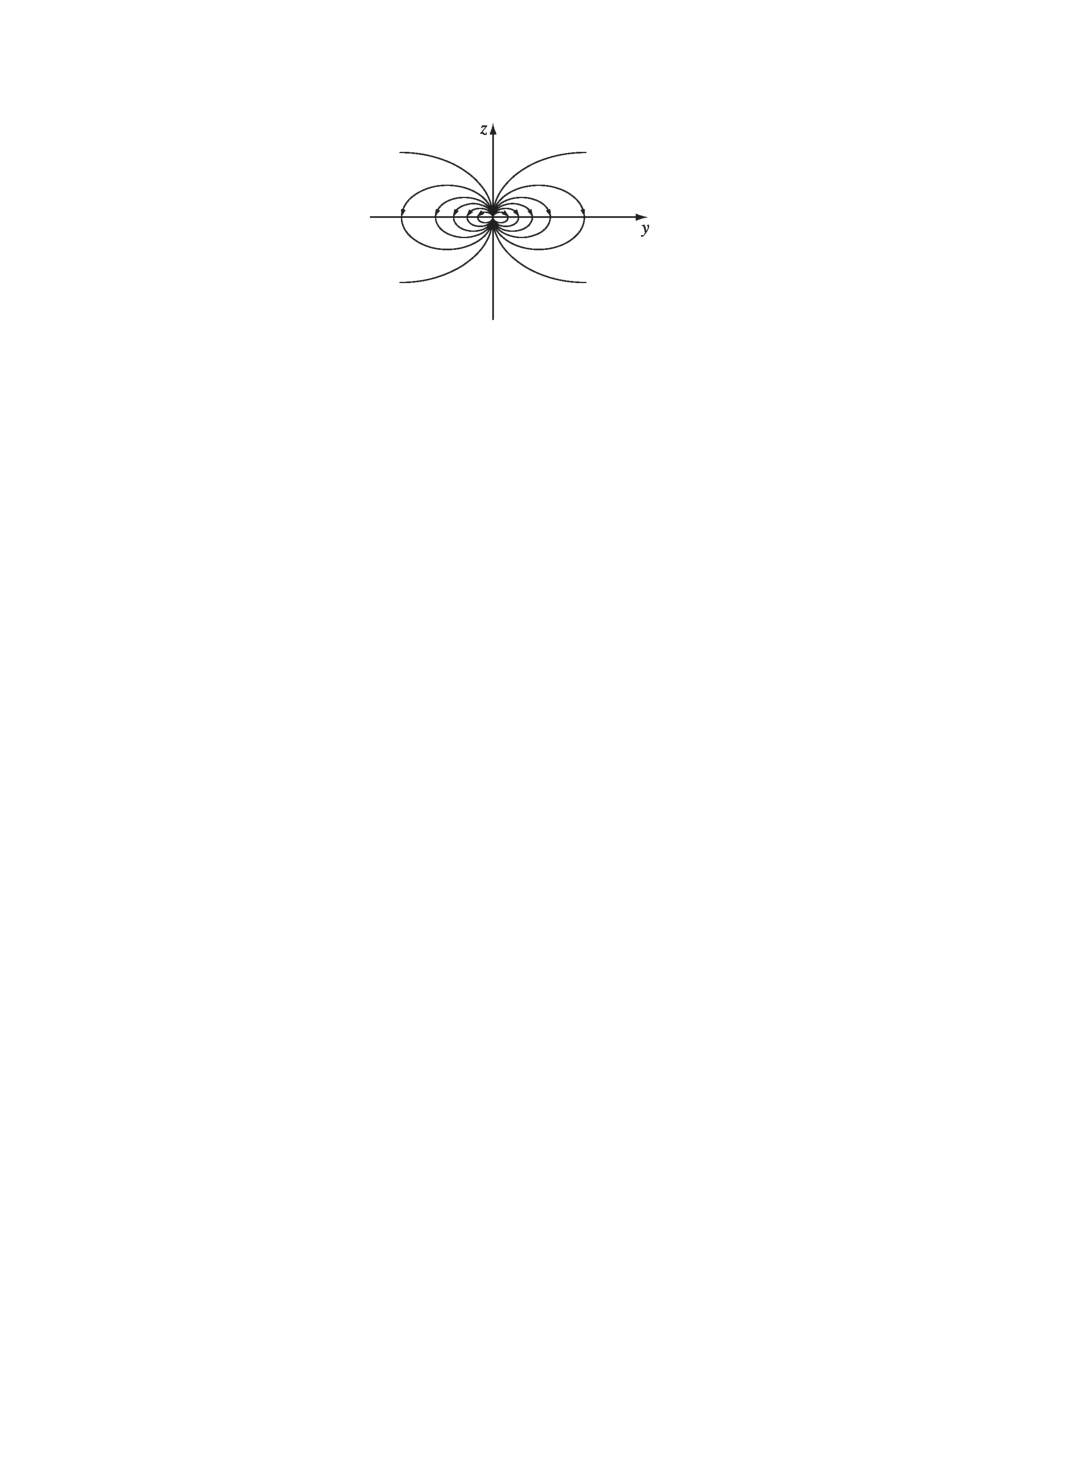
\includegraphics[width=0.4\textwidth]{5-55a}
		\caption{[Griffiths 5.55(a)] The field of a ``pure'' dipole.}
		\label{mag}
	\end{figure}
	
	The parameter $\mu$ is defined by $\mu = \mgam c / \hbar$, where $\mgam$ is the photon mass~\cite[p.~600]{Jackson}.  The earth's radius is $R = \SI{6.37e6}{\meter}$~\cite{YF}, so $\mu < \SI{1.267e-8}{\per\meter}$.  Since $c = \SI{2.998e8}{\meter\per\second}$ and $\hbar = h / (2\pi) = (\SI{6.63e-34}{\joule\second}) / (2\pi) = \SI{1.055e-34}{\joule\second}$~\cite{YF}, we have
	\eq{
		\mgam = \frac{\hbar \mu}{c}
		< \frac{(\SI{1.055e-34}{\joule\second}) (\SI{1.267e-8}{\per\meter})}{\SI{2.998e8}{\meter\per\second}}
		\approx \SI{4e-51}{\kg}
		= \SI{4e-48}{\gram}.
	}
	So the upper bound on the photon mass is \ans{$\mgam < \SI{4e-48}{\gram}$.}
}